\documentclass{article}
\usepackage[utf8]{inputenc}
\usepackage{graphicx}

\usepackage[english]{babel}
\usepackage{hyperref}
\usepackage[final]{pdfpages}
\usepackage{subfig}
\usepackage{booktabs}
\usepackage{siunitx}
\usepackage{amssymb,amsmath,amsthm}
\usepackage{enumitem}
% Math Script Font
\usepackage{mathrsfs}
% For Indicator Variables
\usepackage{bbold}
% Use \mathscr{}



% Sets the paragraph intends and the paragraph spacing.
\setlength{\parindent}{1em}
\setlength{\parskip}{1em}

% Use the library
\usepackage{natbib}
% Use different spacings
\usepackage{setspace}
% Add package for highlights
\usepackage{color,soul}
% Package for landscape
\usepackage{pdflscape}

% Sets the page margins
\usepackage[margin=1in]{geometry}

% Define some shortcuts
\newcommand{\E}{\mathbb{E}}
\newcommand{\R}{\mathbb{R}}

\newcommand{\figog}[4]{\begin{figure}[h!]\caption{#3}\begin{center}\includegraphics[scale={#1}]{#2}\label{#4}\end{center}\end{figure}}


\def\H{\mathbb{H}}
\DeclareMathOperator{\Log}{log}
\DeclareMathOperator{\Min}{min}
\DeclareMathOperator{\Exp}{exp}
\DeclareMathOperator{\Argmin}{argmin}
\DeclareMathOperator{\Argmax}{argmax}
\DeclareMathOperator{\Sup}{sup}
\DeclareMathOperator{\Inf}{inf}

\def\Argmax#1{\underset{\substack{#1}}{\mbox{argmax }}}
\def\argmax{\mbox{arg}\max}
\def\argmin{\mbox{arg}\min}

% Define NEW environments
\newenvironment{enumog}
	{\begin{enumerate}[noitemsep,topsep=0pt,label*=\arabic*.]}{	\end{enumerate}}

	\newenvironment{itemog}
	{\begin{itemize}[noitemsep,topsep=0pt]}{	\end{itemize}}

\begin{document}

\title{Summary Stats}
\author{Oliver Giesecke}


\maketitle 

% NOTE: change system directory first
\begin{table}[h!]
	\begin{center}
		\begin{tabular}{lc}
\hline\hline 
 & Number of Meetings with Bluebooks  \\ 
\hline 
Total & 424 \\ 
In Period 08/13/1968-03/17/2009 & 375 \\ 
...with mentioning of alternative(s) & 333 \\ 
...mentioning of alternative {A} & 293 \\ 
...mentioning of alternative {B} & 327 \\ 
...mentioning of alternative {C} & 288 \\ 
...mentioning of alternative {D} & 20 \\ 
...mentioning of alternative {E} & 1 \\ 
\hline 
\end{tabular}
	\end{center}
\end{table}

\begin{table}[h!]
	\begin{center}
		\begin{tabular}{lccccc}
\hline\hline 
 & Alternative A & Alternative B & Alternative C & Alternative D & Alternative E \\ 
\hline 
Total & 1084 & 1613 & 963 & 90 & 1 \\ 
\addlinespace 
1 & 31 & 14 & 43 & 2 & 1 \\ 
2 & 57 & 30 & 67 & 2 & 0 \\ 
3 & 72 & 50 & 64 & 2 & 0 \\ 
4 & 55 & 64 & 38 & 0 & 0 \\ 
5 & 31 & 63 & 43 & 9 & 0 \\ 
6 & 17 & 32 & 20 & 3 & 0 \\ 
7 & 12 & 29 & 6 & 1 & 0 \\ 
8 & 5 & 18 & 2 & 1 & 0 \\ 
9 & 9 & 11 & 3 & 0 & 0 \\ 
10 & 3 & 7 & 1 & 0 & 0 \\ 
$>10$ & 1 & 9 & 1 & 0 & 0 \\ 
\hline 
\end{tabular}
	\end{center}
\end{table}



\begin{table}[h!]
	\begin{center}
		\begin{tabular}{lc}
\hline\hline 
\addlinespace 
Policy Options & Number of Meetings \\ 
\hline 
E & 3 \\
T & 7 \\
U & 1 \\
U,E & 39 \\
U,T & 57 \\
U,E,T & 61 \\
\addlinespace 
Total & 168 \\
\hline 
\end{tabular}
	\end{center}
\end{table}

\begin{landscape}
\begin{table}[h!]
	\begin{center}
		\begin{tabular}{lcccccccccccccccccccc}
\hline\hline 
\addlinespace 
Policy Options & 1988 & 1989 & 1990 & 1991 & 1992 & 1993 & 1994 & 1995 & 1996 & 1997 & 1998 & 1999 & 2000 & 2001 & 2004 & 2005 & 2006 & 2007 & 2008 & 2009 \\ 
\hline 
E & 0 & 0 & 0 & 0 & 0 & 0 & 0 & 0 & 0 & 0 & 0 & 0 & 0 & 0 & 0 & 0 & 0 & 1 & 3 & 0 \\
T & 5 & 0 & 0 & 0 & 0 & 0 & 1 & 0 & 1 & 0 & 0 & 0 & 1 & 0 & 1 & 5 & 1 & 0 & 0 & 0 \\
T,E & 0 & 0 & 0 & 0 & 0 & 0 & 0 & 1 & 0 & 0 & 0 & 0 & 0 & 0 & 0 & 0 & 0 & 0 & 0 & 0 \\
T,U & 1 & 2 & 1 & 0 & 0 & 0 & 6 & 1 & 3 & 7 & 2 & 7 & 5 & 0 & 5 & 3 & 7 & 1 & 2 & 0 \\
T,U,E & 2 & 4 & 6 & 1 & 7 & 8 & 1 & 5 & 4 & 1 & 3 & 1 & 2 & 0 & 0 & 0 & 0 & 4 & 1 & 0 \\
U,E & 0 & 2 & 1 & 7 & 1 & 0 & 0 & 1 & 0 & 0 & 3 & 0 & 0 & 1 & 0 & 0 & 0 & 2 & 2 & 2 \\
\addlinespace 
Total & 8 & 8 & 8 & 8 & 8 & 8 & 8 & 8 & 8 & 8 & 8 & 8 & 8 & 1 & 6 & 8 & 8 & 8 & 8 & 2 \\
\hline 
\end{tabular}
	\end{center}
\end{table}
\end{landscape}

\clearpage

\begin{landscape}

		\begin{figure}[!htp]
		\begin{center}
	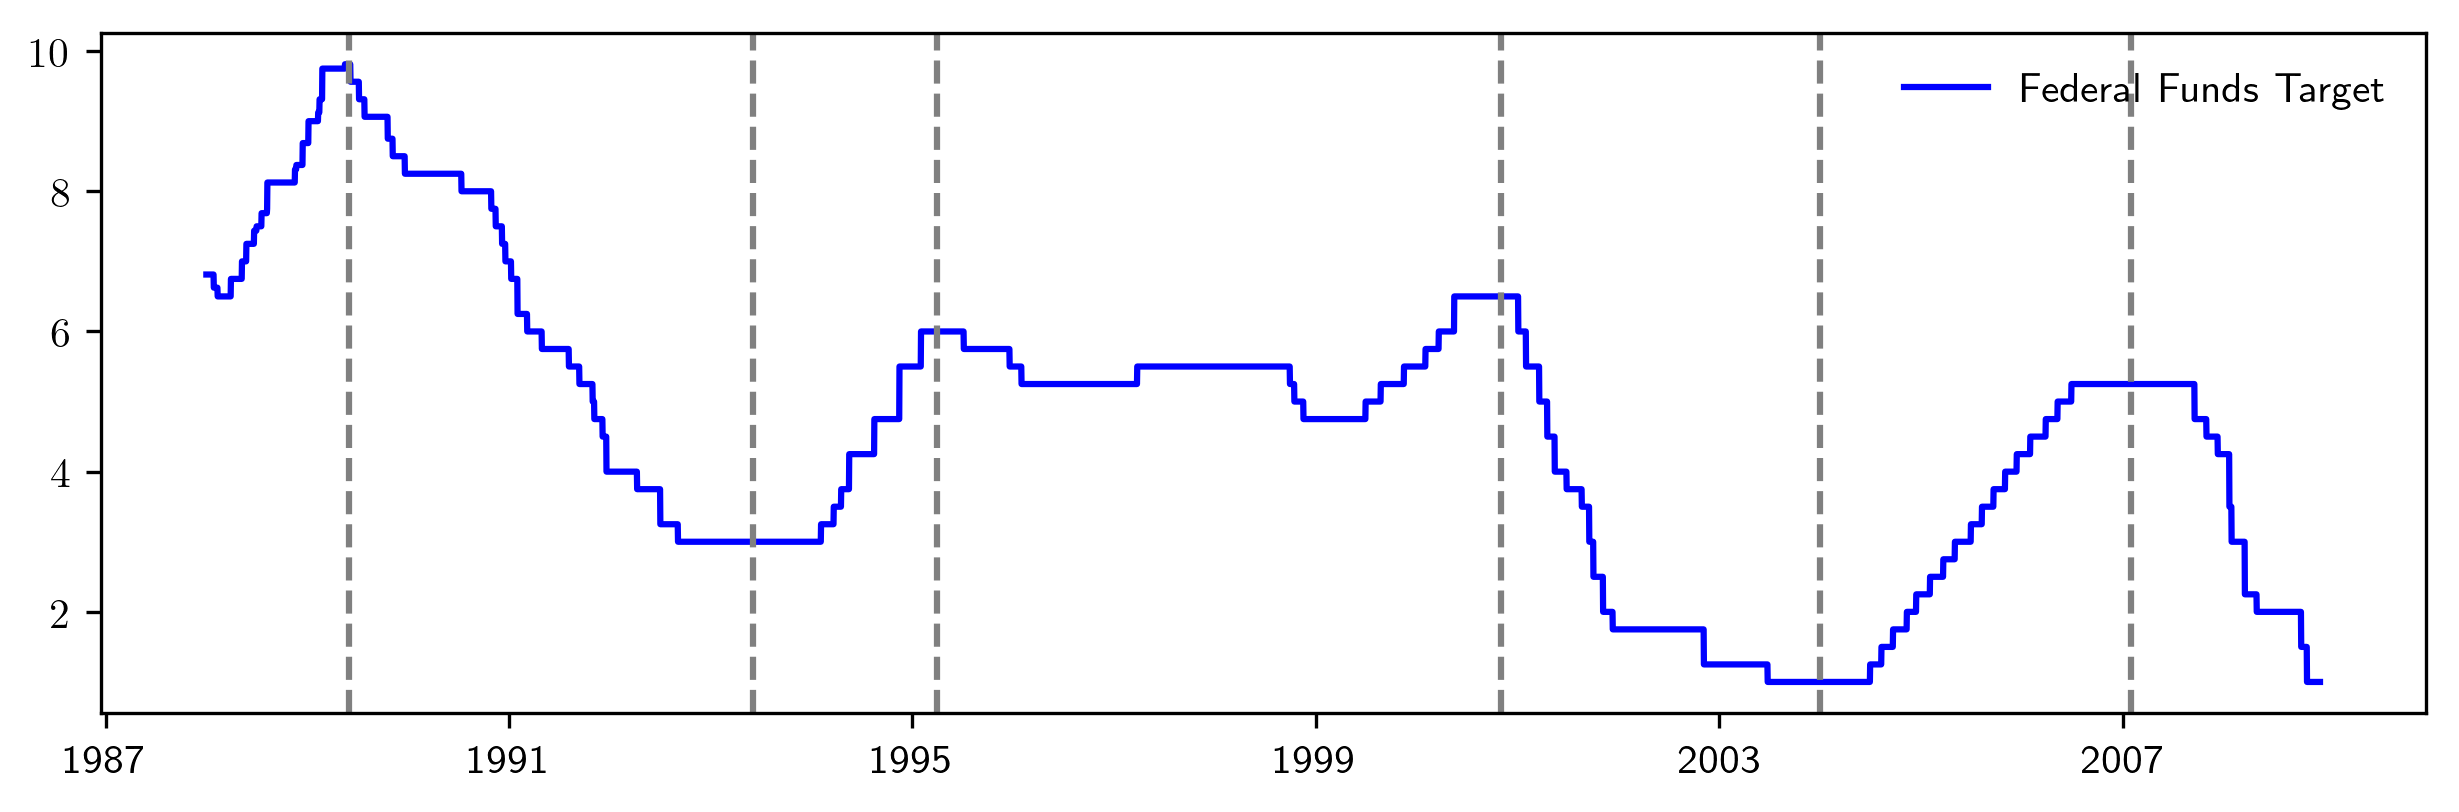
\includegraphics[scale=.95]{../../output/fig_fed_target.png}
		\end{center}
	\end{figure}
	
	\begin{table}[!htp]
		\begin{center}
			\begin{tabular}{lccccccc}
\hline\hline 
\addlinespace 
Policy Options & pre 1989-06-01 & \shortstack{1989-06-01- \\ 1993-06-01} & \shortstack{1993-06-01- \\ 1995-04-01} & \shortstack{1995-04-01- \\ 2000-11-01} & \shortstack{2000-11-01- \\ 2004-01-01} & \shortstack{2004-01-01- \\ 2007-02-01} & post 2007-02-01 \\ 
\hline 
E & 0 & 0 & 0 & 0 & 0 & 0 & 4 \\
T & 5 & 0 & 1 & 2 & 0 & 7 & 0 \\
T,E & 0 & 0 & 0 & 1 & 0 & 0 & 0 \\
T,U & 3 & 1 & 7 & 24 & 0 & 16 & 2 \\
T,U,E & 3 & 20 & 7 & 13 & 2 & 0 & 5 \\
U,E & 0 & 11 & 0 & 4 & 1 & 0 & 6 \\
\addlinespace 
Total & 11 & 32 & 15 & 44 & 3 & 23 & 17 \\
\hline 
\end{tabular}
		\end{center}
	\end{table}
\end{landscape}

\begin{landscape}
	\begin{table}[h!]
		\begin{center}
			\begin{tabular}{lc}
\hline\hline 
\addlinespace 
Policy Options & Number of Meetings \\ 
\hline 
0, 0.5 & 12 \\
0, 0.25 & 21 \\
-0.5, 0 & 12 \\
0, 0, 0 & 1 \\
-0.25, 0 & 11 \\
0.25, 0.5 & 1 \\
0, 0, 0.5 & 1 \\
0.25, 0.25 & 1 \\
0, 0, 0.25 & 6 \\
-0.25, 0, 0 & 2 \\
0, 0.25, 0.5 & 12 \\
-0.25, -0.25 & 1 \\
-0.5, 0, 0.5 & 39 \\
-0.5, 0, 0.25 & 2 \\
-0.5, -0.5, 0 & 1 \\
0, 0.25, 0.25 & 4 \\
-0.25, 0, 0.5 & 2 \\
-0.5, -0.25, 0 & 11 \\
-0.25, 0, 0.25 & 16 \\
0.25, 0.25, 0.5 & 4 \\
0, 0, 0.25, 0.25 & 1 \\
0.25, 0.25, 0.25 & 1 \\
-0.75, -0.5, -0.25 & 2 \\
-1, -0.5, -0.25, 0.0 & 1 \\
-0.5, -0.5, -0.25, 0.0 & 1 \\
-0.75, -0.5, -0.25, 0.0 & 2 \\
\addlinespace 
Total & 168 \\
\hline 
\end{tabular}
		\end{center}
	\end{table}
\end{landscape}

\begin{landscape}
	\begin{table}[h!]
		\begin{center}
			\begin{tabular}{lccccccc}
\hline\hline 
\addlinespace 
Policy Options & pre 1989-06-01 & \shortstack{1989-06-01- \\ 1993-06-01} & \shortstack{1993-06-01- \\ 1995-04-01} & \shortstack{1995-04-01- \\ 2000-11-01} & \shortstack{2000-11-01- \\ 2004-01-01} & \shortstack{2004-01-01- \\ 2007-02-01} & post 2007-02-01 \\ 
\hline 
-0.25, -0.25 & 0 & 0 & 0 & 0 & 1 & 0 & 0 \\
-0.25, 0 & 0 & 0 & 0 & 3 & 8 & 0 & 0 \\
-0.25, 0, 0 & 0 & 0 & 0 & 0 & 1 & 0 & 1 \\
-0.25, 0, 0.25 & 0 & 0 & 0 & 6 & 4 & 1 & 5 \\
-0.25, 0, 0.5 & 2 & 0 & 0 & 0 & 0 & 0 & 0 \\
-0.5, -0.25, 0 & 0 & 0 & 0 & 0 & 9 & 0 & 2 \\
-0.5, -0.5, -0.25, 0.0 & 0 & 0 & 0 & 0 & 0 & 0 & 1 \\
-0.5, -0.5, 0 & 0 & 0 & 0 & 0 & 0 & 0 & 1 \\
-0.5, 0 & 0 & 11 & 0 & 1 & 0 & 0 & 0 \\
-0.5, 0, 0.25 & 0 & 2 & 0 & 0 & 0 & 0 & 0 \\
-0.5, 0, 0.5 & 5 & 19 & 7 & 8 & 0 & 0 & 0 \\
-0.75, -0.5, -0.25 & 0 & 0 & 0 & 0 & 2 & 0 & 0 \\
-0.75, -0.5, -0.25, 0.0 & 0 & 0 & 0 & 0 & 0 & 0 & 2 \\
-1, -0.5, -0.25, 0.0 & 0 & 0 & 0 & 0 & 0 & 0 & 1 \\
0, 0, 0 & 0 & 0 & 0 & 0 & 0 & 1 & 0 \\
0, 0, 0.25 & 0 & 0 & 0 & 0 & 0 & 5 & 1 \\
0, 0, 0.25, 0.25 & 0 & 0 & 0 & 0 & 0 & 1 & 0 \\
0, 0, 0.5 & 1 & 0 & 0 & 0 & 0 & 0 & 0 \\
0, 0.25 & 0 & 0 & 0 & 18 & 1 & 1 & 1 \\
0, 0.25, 0.25 & 0 & 0 & 0 & 0 & 0 & 4 & 0 \\
0, 0.25, 0.5 & 0 & 0 & 4 & 2 & 0 & 6 & 0 \\
0, 0.5 & 3 & 0 & 4 & 5 & 0 & 0 & 0 \\
0.25, 0.25 & 0 & 0 & 0 & 0 & 0 & 1 & 0 \\
0.25, 0.25, 0.25 & 0 & 0 & 0 & 0 & 0 & 1 & 0 \\
0.25, 0.25, 0.5 & 0 & 0 & 0 & 0 & 0 & 4 & 0 \\
0.25, 0.5 & 0 & 0 & 0 & 1 & 0 & 0 & 0 \\
\addlinespace 
Total & 11 & 32 & 15 & 44 & 26 & 25 & 15 \\
\hline 
\end{tabular}
		\end{center}
	\end{table}
\end{landscape}

\begin{table}[h!]
	\begin{center}
		\begin{tabular}{lcccccccccc}
\hline\hline 
\addlinespace 
Available statement & 1988 & 1989 & 1990 & 1991 & 1992 & 1993 & 1994 & 1995 & 1996 & 1997 \\ 
\hline 
No & 12 & 14 & 12 & 19 & 12 & 16 & 7 & 8 & 7 & 7 \\
Yes & 0 & 0 & 0 & 0 & 0 & 0 & 6 & 3 & 1 & 1 \\
\addlinespace 
Total & 12 & 14 & 12 & 19 & 12 & 16 & 13 & 11 & 8 & 8 \\
\hline 
\addlinespace 
Available statement & 1998 & 1999 & 2000 & 2001 & 2002 & 2003 & 2004 & 2005 & 2006 & 2007 \\ 
\hline 
No & 7 & 2 & 0 & 2 & 0 & 5 & 0 & 0 & 0 & 1 \\
Yes & 3 & 6 & 8 & 11 & 8 & 8 & 8 & 8 & 8 & 10 \\
\addlinespace 
Total & 10 & 8 & 8 & 13 & 8 & 13 & 8 & 8 & 8 & 11 \\
\hline 
\addlinespace 
\end{tabular}
	\end{center}
\footnotesize{\textit{Note:} The total number of each column represents the number of meetings and conference call in the respective year. The breakdown shows for how many of these meetings a statement is available.}
\end{table}


\end{document}